%%%%%%%%%%%%%%%%%%%%%%%%%%%%%%%%%%%%%%%%%%%%%%%%%%%%%%%%%%%%%%%%%%%%%%%%%%%%%%%%
%2345678901234567890123456789012345678901234567890123456789012345678901234567890
%        1         2         3         4         5         6         7         8

%\documentclass[letterpaper, 10 pt, conference]{ieeeconf}  % Comment this line out if you need a4paper

\documentclass[a4paper, 10pt, conference]{ieeeconf}      % Use this line for a4 paper

\IEEEoverridecommandlockouts                              % This command is only needed if
                                                          % you want to use the \thanks command

\overrideIEEEmargins                                      % Needed to meet printer requirements.

%In case you encounter the following error:
%Error 1010 The PDF file may be corrupt (unable to open PDF file) OR
%Error 1000 An error occurred while parsing a contents stream. Unable to analyze the PDF file.
%This is a known problem with pdfLaTeX conversion filter. The file cannot be opened with acrobat reader
%Please use one of the alternatives below to circumvent this error by uncommenting one or the other
%\pdfobjcompresslevel=0
%\pdfminorversion=4

% See the \addtolength command later in the file to balance the column lengths
% on the last page of the document

% The following packages can be found on http:\\www.ctan.org
\usepackage{graphics} % for pdf, bitmapped graphics files
\usepackage{epsfig} % for postscript graphics files
\usepackage{mathptmx} % assumes new font selection scheme installed
%\usepackage{times} % assumes new font selection scheme installed
\usepackage{amsmath} % assumes amsmath package installed
\usepackage{amssymb}  % assumes amsmath package installed
%\usepackage{algorithmicx}
%\usepackage[Algorithm,ruled]{algorithm}
%\usepackage{algpseudocode}
\usepackage{tabularx}
\usepackage{multirow}
\usepackage{color}
\usepackage{url}
%\usepackage{balance}
\usepackage{subcaption}
\usepackage{breqn}
\usepackage{algorithm2e}
\usepackage{dblfloatfix} 
\usepackage[export]{adjustbox}
\usepackage{tabulary,booktabs}
%\usepackage{verbatim}
%\usepackage{flushend}

\newcommand{\junk}[1]{}
\newcommand{\abs}[1]{\left| #1 \right|} %| |
\newcommand{\comment}[1]{\textcolor{red}{#1}}



\title{\LARGE \bf
COMP0129: Team 2 Coursework 2 Report 2
}

\author{Ahmed Adamjee$^{1}$, Abdulbaasit Sanusi^{2}$, Kennedy Dike^{3}$% <-this % stops a space
\thanks{$^{1}$Department of Computer Science, University College London, Gower Street, WC1E 6BT, UK.
{\tt\small {Ahmed.Adamjee.21}@ucl.ac.uk}}%
\thanks{$^{2}$Department of Computer Science, University College London, Gower Street, WC1E 6BT, UK.
{\tt\small {Abdulbaasit.Sanusi.21}@ucl.ac.uk}}%
\thanks{$^{3}$Department of Computer Science, University College London, Gower Street, WC1E 6BT, UK.
{\tt\small {Ikedinaekpere.Dike.21}@ucl.ac.uk}}%
}

\date{01 January 2021} %it will not be displayed

\begin{document}

\maketitle
\thispagestyle{empty}
\pagestyle{empty}

\begin{abstract}
This is an example template for the Overleaf documentation.
\end{abstract}

\input{introduction.tex}
\section{BACKGROUND AND LITERATURE REVIEW}\label{Sec:intro}
This is an introduction to $\LaTeX$ for the COMP0219 course.  The basic $\LaTeX$ tricks you may want are the following.  First, make sure that you write all your text in the main.tex.  Whenever you want to check the .pdf file, press the PDF button on the left sidebar and click: Recompile.  Secondly, you should be able to include figures and images in your document, which is done as follows (give always a label):

In Fig.~\ref{Fig:universe} we show a picture of the universe!

\begin{figure}[ht!]
  \centering
  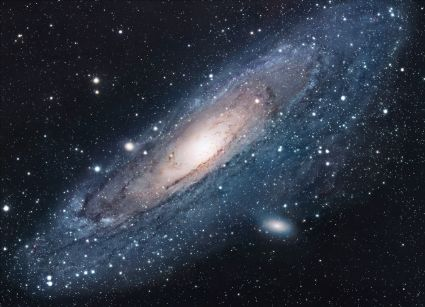
\includegraphics[scale=1.7]{figures/universe.jpg}
  \caption{The Universe}
  \label{Fig:universe}
\end{figure}
\section{PROPOSAL}\label{Sec:method}
In proposed solution, the Spot robot [289] is equipped with additional sensors and the appropriate modules, with respect to the firefighting scenario. A FARO Focus Laser Scanner [https://www.faro.com/en/Products/Hardware/Trek-3D-Laser-Scanning-Integration] is integrated to enable autonomous live scanning of the environment, which can be extremely useful to enable firefighters look at the scene and determine how to enter the scene if a human needs to be rescued once detected. A Probe Microphone ICP [https://www.pcb.com/products?m=377b26] is attached, which can enable us to detect noises from humans calling for help to aid in the detection of life, suitable to operate in the required temperature range. Additionally, a radiometric, FLIRⓇ, thermal camera [https://www.flir.co.uk/products/e6-xt/] is also attached, which detects up to a maximum of 550\degree C., which can be used to infer what are the most impacted regions in the environment, and if a human detected is caught in a fire which can be an immediate concern for firefighters. \\

As described by [8], we add a life detection radar that can sense low frequency pulse of the heart and determine the location of fire victims and survivors. Although they simulated this detector radar in their work, we incorporated a commercially available alternative (lifelocator IV[290]) that works based on the same principle and performs the same functionality. This is then shared along with the live map of the environment to fire fighters and be used by the fire fighter to rescue trapped victims.\\

We have included a suction vacuum fan on the back of the robot, along with a commercially available $\mathrm{CO_2}$ sensor[10][11]. This is such that the robot can use it to suck out dangerous vapour that could be imminently fatal to people trapped in the environment, based on the gas concentration detected. The robots will need to return outside the building if it is low on battery or needs to empty its fume tank. It can use the map of the environment built to navigate back outside. These modules will need to be designed in such a way that they can be simply swapped without wasting time, especially due to this being an emergency scenario and wasting time charging the robot may not be feasible. The spot robot will be fitted with slide-able slots for the extinguisher which connects it to the actuation mechanism. Fortunately, the Spot robot secures the battery through a simple latch, and a spare battery can be swapped through a sliding mechanism to fulfil our requirements [Reference]. \\

To counteract issues relating to the robot’s operating temperature, it will need to be custom built with thermally resistant materials,aluminium compound metal with Teflon wiring, described in [12], so that it can withstand the heat and function optimally.\\

We propose the robot operates in the stages as follows:
\begin{enumerate}
    \item Evaluate the scenario and send robot to the most affected region.
    \item Use thermal sensor to determine the hottest regions
    \item Advance towards hottest region; If path blocked, use arm to remove obstacles in the way to allow for a clear rescue path, by utilising Exteroceptive sensors (RGB camera) and Proprioceptive sensors (IMU), on the manipulator.
    \item Detect life using noise detection and life detection sensors
    \item Measure the toxicity of fatal fumes around the trapped person, and suction the fumes according to set threshold
    \item Send the location of detected person along with the generated scan of the environment to the rescue team.
\end{enumerate}

We monitor the level of the fume tank using a pressure sensor and the robot’s battery voltage to determine if the robot needs to return to swap these parts, in which case the robot uses the map it generated of its environment to return outside the building, and later returns to the same location in the building to resume its search and aid operation. 
A diagram of the modified robot is shown in figure X.




% \subsection{Sections and subsections}\label{Sec:general}
% You can split a section to subsections, and even reference them.  For instance Section~\ref{Sec:intro} is the introduction.  You can also reference the figures.  For instance Fig.~\ref{Fig:universe} is a picture of the universe.  Note that you should upload a figure/picture in the same folder and the main.tex file (using the upload button in the left sidebar).  Also you can add references, which have a special format stored in references.bib file.  To reference a paper you can do in the following way: paper~\cite{Adams1995, Kanoulas2019} talks about the universe.

% \subsection{Math}
% Math text in $\LaTeX$ are going between dollar signs: $^{0}T_{1}$ is a transformation from frame ${1}$ to frame ${2}$.  The underscore is for subscripts and the hat for superscripts, i.e. $a^2$ and $b_2$.  Also we can include a bit more complex equations in the following way:

% \begin{equation}
%     ^{0}T_{1} =
%     \begin{bmatrix}
%     &           & &           \\
%     & ^{0}R_{1} & & ^{0}t_{1} \\
%     &           & &           \\
%     0 & 0 & 0 & 1
%     \end{bmatrix}
% \end{equation}

\section{HYPOTHESIS AND EVALUATION}\label{Sec:concl}
As mentioned earlier in the paper, during evacuation of found humans in a fire outbreak, there poses a risk of worsening the case of the remaining humans who are stuck in the fire. Incorporating our robot in this scenario would identify humans left in the fire, using the LDR, while reducing the amount of fire still present and members of the rescue team take out found humans. The incoporation of this robot should improve overall rescue time as the fire fighter no longer need to restart search procedures after each evacuation as the robot constantly alerts them of the locations of humans, through the LDR, on the map. Furthermore, more lives would potentially be saved as reducing the time would reduce the effect of lack of oxygen due to the fire. \\

During fire fighting training, fire fighters often train in a controlled environment which is
set on fire in order to simulate actual scenarios. In this process, the fire fighters are expected to search for and evacuate all "dummy" humans captured in the burning area as well as put out the fire. To assess the impact the robots have on the fire fighting process, an experiment can be designed such that the fire fighting team would complete the controlled live-fire training scenario with and without the aid of the robot.To make the dummies identifiable by the LDR, heartbeats and respiratory signals of test humans would be prerecorded and put in a "transmitter", inserted into the body of the dummies. This would mimic the presence of humans to the LDR on the robot as it would detect those signals. Furthermore, speakers, which would expel human-like noises, would also be inserted into few of the dummies.\\

The robot is going to be evaluated based on a number of key performance indicators. This indicators essentially highlight the extent of aid the robot provides to the fire fighting team. These performance indicators are:
\begin{enumerate}
    \item Ability to detect survivors/victims: The robot should be able to identify all humans in the burning area
    \item Accuracy of the map of the area: The map has to be accurate enough as the locations of survivors would be placed on the map created by the robot
    \item Time taken to complete process with and without the aid of the robot: The time taken to complete the process with the robot should be considerably lower than without  using the robot.
    \item How effective is the robot in identifying and putting out fires
\end{enumerate}


% I will keep this document updated when new techniques are needed.  Google is always there for you to find the right way to write in $\LaTeX$, although you can also read any $\LaTeX$ Cheat Sheet, e.g.\\ \url{https://www.nyu.edu/projects/beber/files/Chang_LaTeX_sheet.pdf}

\section{CONCLUSIONS AND FUTURE WORK}\label{Sec:concl}
I will keep this document updated when new techniques are needed.  Google is always there for you to find the right way to write in $\LaTeX$, although you can also read any $\LaTeX$ Cheat Sheet, e.g.\\ \url{https://www.nyu.edu/projects/beber/files/Chang_LaTeX_sheet.pdf}


\bibliographystyle{IEEEtran}
\bibliography{references}
\end{document}